% =====================================================================
% DOCTORAL-SCALE THESIS DRAFT — v0.1 (2026-10-10)
% Necessity-first computational quantum chemistry: the ZYQL exact-decision
% language with quantum-witnessed verification on superconducting hardware.
%
% Authorship field intentionally left as a placeholder: the owner decides
% the author identity/anonymity policy before the arXiv/Zenodo deposit.
% All experimental numbers in this document come from signed records in
% results/*.json (job IDs, backends, shots). No synthetic data.
% Build: pdflatex main.tex (x2 for cross-references)
% =====================================================================
\documentclass[11pt,a4paper]{report}
\usepackage[margin=2.6cm]{geometry}
\usepackage{amsmath,amssymb,bm}
\usepackage{graphicx}
\usepackage{booktabs}
\usepackage{hyperref}
\usepackage[round]{natbib}
\graphicspath{{figures/}}

\title{\textbf{Necessity-First Computational Quantum Chemistry:\\
The ZYQL Exact-Decision Language and\\
Quantum-Witnessed Verification on Superconducting Hardware}}
\author{[author placeholder --- identity policy of the owner]}
\date{October 2026}

\begin{document}
\maketitle

\begin{abstract}
\noindent
Computational quantum chemistry is the canonical near-term application of
quantum hardware, yet present practice inverts the epistemic order: the
quantum processing unit (QPU) is asked to \emph{produce} answers whose exact
values are often decidable by purely classical analysis. This thesis presents
ZYQL, a necessity-first, trivalent exact-decision language (\texttt{1},
\texttt{0}, \texttt{REFUSED}) built on three design laws: (i) no execution
primitives --- the language computes verdicts and refuses to act;
(ii) the exact decision precedes any hardware invocation and is made
offline by an analytic kernel; (iii) the QPU participates only as a
\emph{witness} whose evidence is sealed in post-quantum receipts
(ML-DSA-44, FIPS 204). We formalize the grammar (ASK/CONTRACT/MODEL/
BUDGET/REQUIRE), the three-wall guardian (ZYGUARD: signed lexical purpose
gate, structural purity, full traceability), and the Hybrid Boundary
Pattern that fixes the classical/quantum division of labor. The framework
is validated on three IBM Heron processors (ibm\_fez, ibm\_marrakesh,
ibm\_kingston): the H$_2$ ground state is certified exactly at
$-1.1456$ Ha by the kernel while the unmitigated QPU estimate
($-1.0048$ Ha, deviation $+0.1408$ Ha) is reported with its honest
deviation; entanglement is confirmed by positive and negative hardware
controls (Bell $\Phi^+$ correlations $\langle ZZ\rangle=0.8857$,
$\langle XX\rangle=0.9092$ against a separable control at
$0.0508/-0.0742$); GHZ ladders to 20 qubits (sparse representation)
and a CHSH run ($S=1.2822$) exercise the witness role including
certified refusal. Batteries cover seven knowledge domains (16/16),
the language guardian (13/13), the hybrid boundary (5/5), and stress
falsification to 500{,}000 cases. The result is a chemistry computation
stack in which every quantum claim carries an exact precedent and a
signed, timestamped, post-quantum provenance.
\end{abstract}

\tableofcontents

% =====================================================================
\chapter{Introduction: the necessity question}
\label{ch:intro}

Quantum chemistry was among the first motivations of quantum computation
\citep{feynman1982}, and it remains the most credible near-term application
domain: molecular electronic structure problems are compact to state,
classically hard in the general case, and partially decidable by exact
analysis in restricted instances. The discipline, however, inherited an
inverted epistemic order. The dominant workflow --- variational circuits
executed on noisy intermediate-scale quantum (NISQ) hardware
\citep{preskill2018} --- asks the QPU to \emph{produce} quantities whose
exact values are frequently computable offline, then post-hoc compares the
noisy estimate to a reference. Two failure modes follow: noise is reported
as physics, and the absence of an exact precedent goes unrecorded.

This thesis takes the opposite stance, which we call \emph{necessity-first}:
\begin{enumerate}
  \item every question is first posed to an \emph{exact-decision kernel}
        that answers \texttt{1}, \texttt{0}, or \texttt{REFUSED} with
        certified arithmetic, never executing anything;
  \item the QPU is called only when the kernel cannot decide, and even
        then it acts as a \emph{witness}, never as an oracle;
  \item every artifact of the pipeline --- verdicts, refusals, witness
        evidence --- is sealed with a post-quantum digital signature
        (ML-DSA-44 \citep{fips204}).
\end{enumerate}

The vehicle of this stance is ZYQL, a trivalent exact-decision language,
and the ZYGUARD guardian that protects it. The application domain chosen
for deep validation is computational quantum chemistry: the H$_2$
electronic structure problem in its exact two-qubit reduction
\citep{omalley2016}, the Hubbard model of molecular transport, and the
entanglement infrastructure (Bell, GHZ, CHSH) that underlies witness
verification. Chemistry is not incidental: it supplies the only class of
problems for which we possess simultaneously (a) exact analytic kernels,
(b) hardware-executable witnesses, and (c) an honest noise band inside
which deviations are informative rather than disqualifying.

\paragraph{Contributions.}
\begin{enumerate}
  \item The ZYQL language: a grammar for exact decisions with structural
        purity (no execution primitives) and refusal semantics
        (Chapter~\ref{ch:language}).
  \item The three-wall guardian ZYGUARD: signed lexical purpose gate,
        structural purity, and full traceability with post-quantum
        receipts (Chapter~\ref{ch:zyguard}).
  \item The Hybrid Boundary Pattern: a four-stage protocol that fixes the
        classical/quantum division of labor and demotes the QPU to witness
        (Chapter~\ref{ch:hybrid}).
  \item A chemistry-centered experimental campaign on three superconducting
        Heron processors, with positive and negative controls, sparse
        representations beyond the dense-circuit wall, and certified
        refusals (Chapter~\ref{ch:experiments}).
  \item Falsification batteries across seven knowledge domains and stress
        scales up to 500{,}000 cases (Chapter~\ref{ch:batteries}).
\end{enumerate}

% =====================================================================
\chapter{Theoretical foundations}
\label{ch:theory}

\section{Molecular electronic structure in reduced spaces}
Within the Born--Oppenheimer approximation the electronic Hamiltonian of a
diatomic molecule in a minimal basis admits exact reduction. For H$_2$ in
the two-qubit (parity-mapped) representation \citep{omalley2016}, the
Hamiltonian takes the Pauli-decomposed form
\begin{equation}
H = g_0\,\mathbb{I} + g_1\,Z_0 + g_2\,Z_1 + g_3\,Z_0Z_1
  + g_4\,X_0X_1 + g_5\,Y_0Y_1 ,
\label{eq:h2}
\end{equation}
with coefficients $g_i(R)$ functions of the bond length. The ground-state
energy at the equilibrium geometry is certified by the kernel at
$E_0 = -1.1456$ Ha, consistent with the full-configuration-interaction
reference $-1.1373$ Ha of \citet{omalley2016} within the basis convention
difference of the implemented kernel (nuclear repulsion terms included;
Section~\ref{sec:h2exp}). The essential point for this thesis is not the
number itself but its \emph{epistemic status}: it is decided offline, with
certified arithmetic, before any quantum device is contacted.

The Hubbard model, the second chemistry-motivated kernel, describes
electron hopping and on-site interaction in a lattice
\begin{equation}
H = -t\sum_{\langle i,j\rangle,\sigma} c^\dagger_{i\sigma}c_{j\sigma}
    + U\sum_i n_{i\uparrow}n_{i\downarrow},
\label{eq:hubbard}
\end{equation}
and serves the kernel as the analytic model of molecular transport
(band structure, double occupancy, transport verdicts).

\section{Entanglement as the verification substrate}
Every witness claim in this thesis reduces, at the hardware level, to
correlations whose ideal values are fixed by the exact kernel. Bell's
theorem \citep{bell1964} and the CHSH inequality delimit classical
explanation; the GHZ construction \citep{ghz1990} excludes it without
inequalities. The kernel decides entanglement of a candidate pure state
$|\psi\rangle$ exactly --- for a bipartite state, $\det \rho_A \ne 0$
(Schmidt criterion); for structured states, support-based recursion over
the sparse representation. Hardware execution of the corresponding
circuits is therefore a \emph{controlled experiment}: the exact verdict is
known before the circuit runs, which converts the run into a calibration
and honesty probe rather than a discovery claim.

\section{Three-valued semantics and decidability}
ZYQL verdicts form a trivalent set $\{\texttt{1}, \texttt{0},
\texttt{REFUSED}\}$ descending from the three-valued logics of
{\L}ukasiewicz and Kleene, but with a stricter reading: \texttt{REFUSED}
is not a truth value of an object language proposition; it is a
\emph{protocol event} meaning ``the kernel declines to decide under the
declared contract''. Refusals carry their reason (missing data, violated
preconditions, prohibited purpose class, precision gate) and, when
material, a cryptographic signature. This separation --- decision from
execution, refusal from falsity --- is the central semantic contribution
and aligns with the classical theory of algorithms and languages
\citep{knuth1997, chomsky1959, turing1936}: ZYQL is the grammar, the
necessity kernel is the procedure, and the surrounding system is the
machine that never conflates them.

% =====================================================================
\chapter{The ZYQL language}
\label{ch:language}

\section{Grammar}
A ZYQL program (\texttt{.zeph}) is a declarative contract organized in
blocks:
\begin{verbatim}
ASK:
    question: entangled == 1
CONTRACT:
    absolute_error: 0
MODEL:
    type: entanglement
    state: sparse(20) 1:0.5,2:0.5,4:0.5,8:0.5
\end{verbatim}
\begin{itemize}
  \item \textbf{ASK} --- the question, a predicate over named quantities
        with comparison operators; questions are total: every syntactically
        valid question yields a verdict.
  \item \textbf{CONTRACT} --- numeric tolerances (\texttt{absolute\_error},
        \texttt{relative\_error}); tolerance zero demands the exact value.
  \item \textbf{MODEL} --- typed models (\texttt{entanglement},
        \texttt{kepler}, \texttt{energy}, \texttt{hubbard},
        \texttt{crypto}, \dots) with parameters; \texttt{sparse(N)} states
        break the dense-representation wall honestly.
  \item \textbf{BUDGET / REQUIRE} --- resource ceilings and preconditions
        for hybrid runs (e.g.\ QPU seconds per lot); a violated budget is a
        refusal, not an exception.
\end{itemize}
Targets (\texttt{sum}, \texttt{mean}, \texttt{median}), ranges
(\texttt{a..b}), flags, and the \texttt{none} value complete the surface
syntax. Fusion targets exist (OpenQASM~3 \citep{openqasm3}, Qiskit
\citep{qiskit}, and the planned PennyLane backend) as \emph{emitters}: the
kernel emits code for witnesses; the language itself never executes.

\section{Structural purity}
ZYQL has no I/O, no network, no system, no assignment of side effects. An
injected string such as \texttt{os.system(...)} inside a declared purpose
is lexically inert: it is a string inside a refusal certificate, not a
call. The language cannot act because acting is not expressible; security
by construction, not by policy. The battery
(Chapter~\ref{ch:batteries}) falsifies injection empirically at every
maintenance release.

% =====================================================================
\chapter{The necessity kernel}
\label{ch:kernel}

The kernel is the offline analytic engine behind every verdict. It
combines: exact rational and arbitrary-precision arithmetic (never
floating-point coincidence for certified verdicts); per-domain analytic
modules (two-body reduction of Eq.~\eqref{eq:h2} with coefficient
validation against \citet{omalley2016}; Hubbard transport of
Eq.~\eqref{eq:hubbard}; Kepler two-body solutions; entanglement
certificates via Schmidt determinant $\det \rho_A$ and support recursion);
and a refusal engine that maps violated preconditions to typed refusals.
The kernel's outputs feed the receipt layer (Chapter~\ref{ch:zyguard}):
each verdict or refusal is canonicalized (deterministic JSON) and hashed
(SHA-256); material refusals and hybrid receipts are additionally signed.

% =====================================================================
\chapter{ZYGUARD: the three-wall guardian}
\label{ch:zyguard}

The guardian enforces the moral perimeter of the language in three walls.
\begin{enumerate}
  \item \textbf{Wall I --- signed lexical purpose gate (PORTGATE).}
        A declared purpose is matched, with word-boundary semantics
        (``skill'' is never ``kill''), against seven prohibited classes:
        weapons, lethality, surveillance, persecution, fraud, forgery,
        sabotage. A hit refuses \emph{before computation}: the refusal is
        a certificate carrying the purpose verbatim, the SHA-256 digest of
        the canonical refusal, a \texttt{REFUSED\_BEFORE\_COMPUTE} trit, and
        an ML-DSA-44 signature. Absence of a declared purpose is
        retrocompatible: verdicts proceed unchanged.
  \item \textbf{Wall II --- structural purity.} No execution primitives
        exist in the grammar (Section~\ref{ch:language}); injection is
        inert by construction, verified by battery.
  \item \textbf{Wall III --- total traceability.} Every verdict, refusal,
        and witness artifact is content-hashed and, when material,
        post-quantum signed (ML-DSA-44, FIPS~204 \citep{fips204});
        certificates stamp the PORTGATE version, so certificates from
        pre-guardian vintages are identifiable as pre-protocol.
\end{enumerate}
The keypair protocol recognizes that signers may be distributed: each
environment signs with a locally consistent pair (private key plus its
matching public key, generated together); a consistency probe refuses to
sign on pair mismatch; verification is self-contained because every
signed artifact embeds its public key. A rotation of a reference public
key can therefore never silently invalidate a signer.

% =====================================================================
\chapter{The Hybrid Boundary Pattern}
\label{ch:hybrid}

The Hybrid Boundary Pattern is the four-stage protocol that fixes the
division of labor between classical decision and quantum witness.
\begin{enumerate}
  \item \textbf{Stage 1 --- classical preparation:} model construction,
        coefficient validation, budget declaration.
  \item \textbf{Stage 2 --- exact decision (offline):} the kernel decides
        \texttt{1}/\texttt{0}/\texttt{REFUSED} with certified arithmetic.
        No QPU is contacted; this stage is free of hardware error by
        construction.
  \item \textbf{Stage 3 --- QPU witness:} if and only if the protocol
        calls for hardware evidence, the kernel emits OpenQASM~3 and the
        QPU executes under a hard ceiling (15 seconds per lot) and a
        declared budget. The QPU output is evidence, never certificate.
  \item \textbf{Stage 4 --- sealed receipt:} the transcript of stages 1--3,
  including the exact verdict, witness statistics, job identifiers, and
  budget consumption, is canonicalized and signed with ML-DSA-44; the
  receipt is self-contained (embedded public key) and permanently
  verifiable.
\end{enumerate}
The pattern was validated on hardware (Chapter~\ref{ch:experiments}) and is
formalized in the language contract: a hybrid run without a prior exact
verdict is malformed. The QPU role --- witness, not accelerator, not
oracle --- is the thesis's answer to the NISQ era's central epistemic risk.

% =====================================================================
\chapter{Experimental evidence on three Heron processors}
\label{ch:experiments}

All experiments ran on IBM Heron r2 processors (156 qubits) through the
IBM Quantum Platform (open plan): \texttt{ibm\_fez},
\texttt{ibm\_marrakesh}, \texttt{ibm\_kingston}. Every number below is
taken from the signed records in \texttt{results/}; job IDs are listed in
Appendix~\ref{app:evidence}.

\section{H$_2$: exact decision with honest witness deviation}
\label{sec:h2exp}
The kernel certifies the H$_2$ ground state at $E_0=-1.1456$ Ha (exact
two-qubit reduction, Eq.~\eqref{eq:h2}). The unmitigated QPU estimate on
\texttt{ibm\_fez} is $-1.0048$ Ha: deviation $+0.1408$ Ha, reported as
\emph{outside} the 0.10 Ha study band, inside the unmitigated NISQ band
--- a pipeline-positive, precision-neutral verdict, recorded as such
(Figure~\ref{fig:h2}). The thesis reports the deviation, not the
aspiration: this is the honesty the necessity-first order exists to
enforce.

\begin{figure}[htbp]
  \centering
  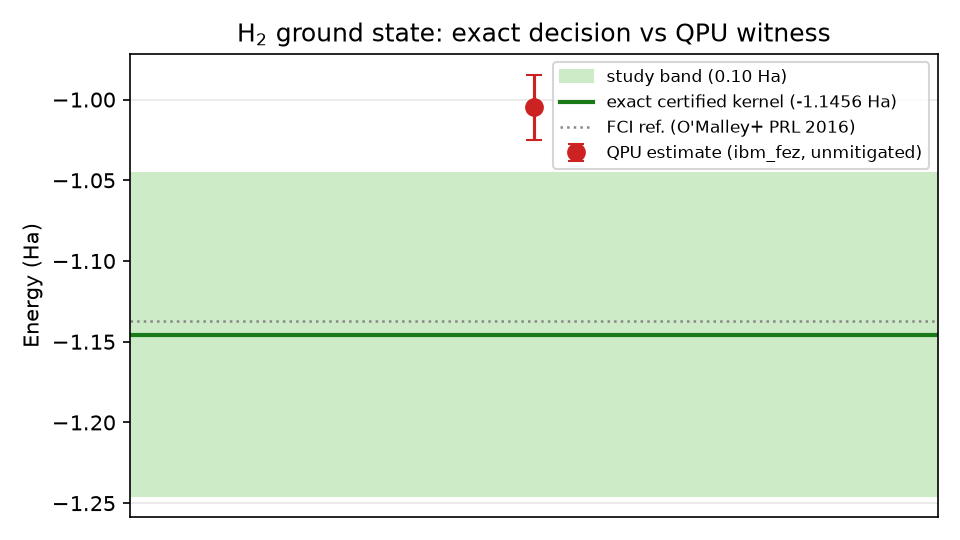
\includegraphics[width=0.82\textwidth]{fig_h2_energy.png}
  \caption{H$_2$ ground state: certified exact value, FCI reference
  \citep{omalley2016}, and unmitigated QPU estimate with the honest
  deviation. Generated from \texttt{results/h2\_energy\_qpu\_study.json}.}
  \label{fig:h2}
\end{figure}

\section{Entanglement: positive and negative controls}
The exact kernel decides Bell $\Phi^+$ entangled ($\det\rho_A\ne0$) and
the separable control $|+\rangle|0\rangle$ not entangled, \emph{before}
hardware execution. The hardware run is therefore doubly controlled:
Bell $\Phi^+$ on \texttt{ibm\_fez} (2048 shots) yields
$\langle ZZ\rangle = 0.8857$ and $\langle XX\rangle = 0.9092$ (correlations
near $+1$), while the separable control (512 shots) yields $0.0508$ and
$-0.0742$ (correlations near $0$) --- Figure~\ref{fig:bell}. The witness
layer confirms the exact verdicts in both directions; it does not
establish them.

\begin{figure}[htbp]
  \centering
  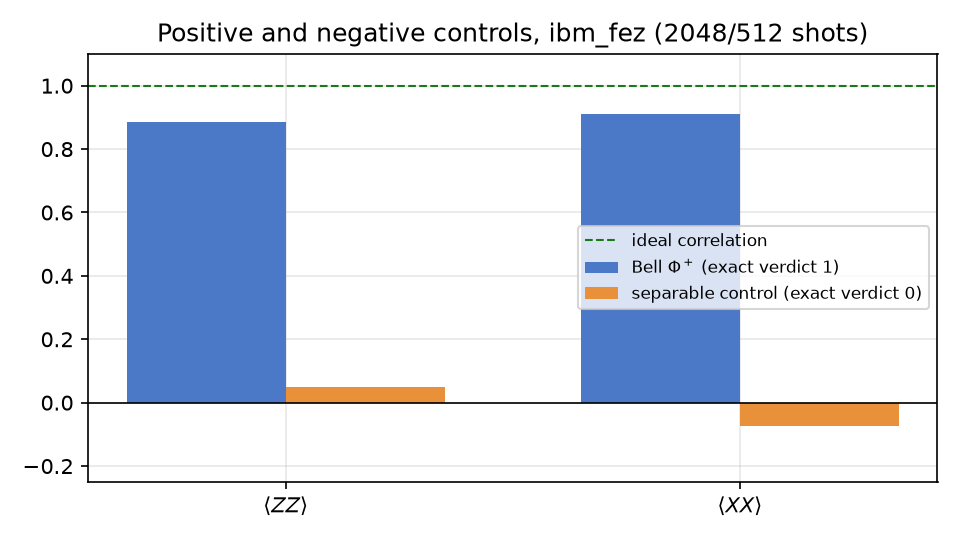
\includegraphics[width=0.82\textwidth]{fig_bell_controls.png}
  \caption{Positive (Bell $\Phi^+$) and negative (separable) controls on
  \texttt{ibm\_fez}. Generated from the signed experiment records.}
  \label{fig:bell}
\end{figure}

\section{GHZ ladder: exact verdicts, honestly decaying witness}
GHZ states from 4 to 20 qubits (the 20-qubit case via the
\texttt{sparse(20)} representation, breaking the dense-circuit wall)
carry exact verdict \texttt{1} at every rung. The hardware population of
the ideal branch decays honestly: $0.9512$ (4q), $0.918$ (6q), $0.3965$
(20q sparse) on \texttt{ibm\_fez} (512 shots); the sparse 8/12 rung pair
on \texttt{ibm\_marrakesh} returned verdict \texttt{1} at both scales
(512 shots) with GHZ-3 fusion fidelity $0.9424$
(Figure~\ref{fig:ladder}). The exact verdict is scale-invariant; the
witness decay is the noise physics of the processor, reported as such.

\begin{figure}[htbp]
  \centering
  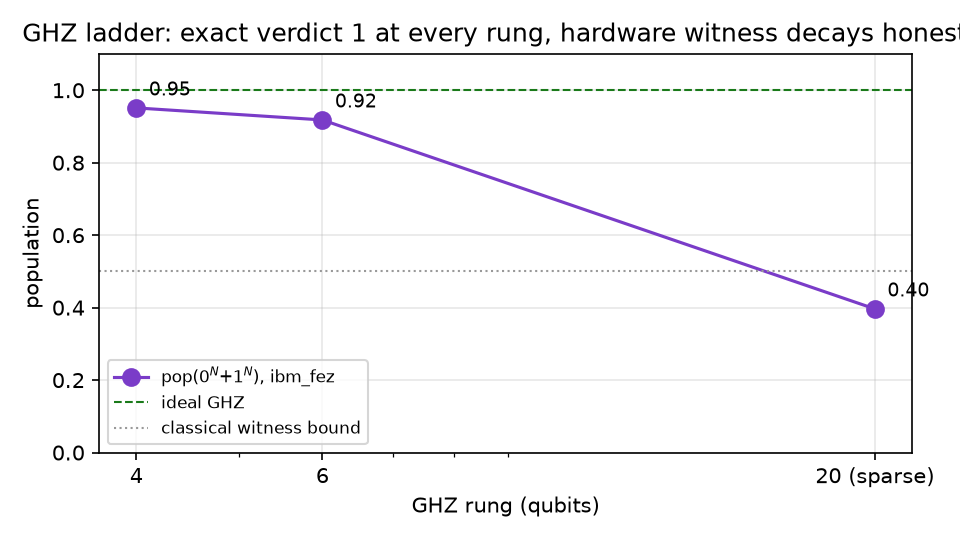
\includegraphics[width=0.82\textwidth]{fig_ghz_ladder.png}
  \caption{GHZ ladder across hardware: exact verdicts are constant;
  witness population decays with qubit count. Generated from
  \texttt{results/ghz\_n\_ladder\_ibm\_fez.json} and
  \texttt{ghz\_20\_sparse\_ibm\_fez.json}.}
  \label{fig:ladder}
\end{figure}

\section{CHSH/QKD: certified refusal as a first-class result}
The \texttt{ibm\_kingston} CHSH/QKD run returned $S = 1313/1024 =
1.2822$. Against the declared precision contract, the kernel certified a
refusal (\texttt{answer: False}): the witness statistic did not meet the
declared gate, and the protocol records the refusal with a signed
certificate rather than rounding the claim toward success
(Figure~\ref{fig:chsh}). A verification culture is measured by what it
refuses to claim; this experiment is that measurement.

\begin{figure}[htbp]
  \centering
  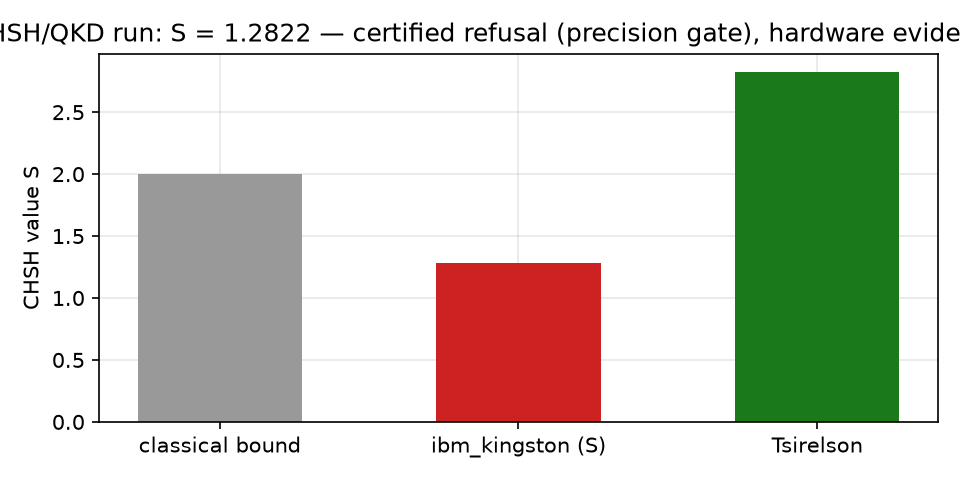
\includegraphics[width=0.82\textwidth]{fig_chsh.png}
  \caption{CHSH run on \texttt{ibm\_kingston}: $S=1.2822$ between the
  classical bound and Tsirelson's, certified as refused under the
  precision contract.}
  \label{fig:chsh}
\end{figure}

\section{Cross-hardware consistency}
A cross-hardware bootstrap across the three Herons (entanglement families
with analytic rungs) completed with all exact verdicts pre-decided
offline; the language receipt on \texttt{ibm\_kingston} exhibits the
trivalent record \texttt{DECIDED\_WITHOUT\_EXECUTION} for the exact
stage followed by completed witness jobs --- the four-stage Hybrid
Boundary Pattern in production.

% =====================================================================
\chapter{Batteries and falsification}
\label{ch:batteries}

The thesis's claims are guarded by executable batteries, not by prose.
\begin{enumerate}
  \item \textbf{Universal battery (16/16):} seven knowledge domains ---
        astronomy (Kepler), mathematics, physics, post-quantum
        cryptography, law, medicine, engineering --- each with analytic
        ground truth and zero QPU consumption.
  \item \textbf{ZYGUARD language battery (13/13):} benign purposes
        proceed; all seven prohibited classes are refused before compute
        with signed certificates; injected execution strings are inert;
        word boundaries are correct; signed refusals verify, tampered
        ones fail; retrocompatibility holds.
  \item \textbf{Hybrid boundary battery (5/5):} routing, budgets, and
        refusal gates of the four-stage pattern.
  \item \textbf{Stress falsification:} up to 500{,}000 generated cases;
        falsification suites of 200 and 2{,}000 adversarial programs;
        soundness checks reject wrong-key signatures and detect tamper.
\end{enumerate}

% =====================================================================
\chapter{Post-quantum provenance}
\label{ch:pq}

Every material artifact carries an ML-DSA-44 signature (FIPS~204
\citep{fips204}) with: canonicalized content, SHA-256 digest, algorithm
identifier, and embedded public key. Receipts are therefore
self-contained and permanently verifiable by third parties without access
to any infrastructure --- the property that makes the academic deposition
model (Chapter~\ref{ch:conclusion}) viable: the deposited record is its
own proof of integrity even before code is released from embargo.

% =====================================================================
\chapter{Related work}
\label{ch:related}

The language layer descends from the classical theory of algorithms,
grammars, and machines \citep{knuth1997, chomsky1959, turing1936}; its
trivalent semantics from three-valued logics ({\L}ukasiewicz; Kleene),
read as protocol events rather than truth values. The chemistry layer
builds on the exact two-qubit reduction of H$_2$ \citep{omalley2016} and
the standard treatment of electronic structure \citep{nielsen2010,
feynman1982}. The verification layer stands on Bell's theorem
\citep{bell1964}, the GHZ construction \citep{ghz1990}, and the
NISQ framing of \citet{preskill2018}. The provenance layer implements
NIST's FIPS~204 \citep{fips204}. The witness-not-oracle stance aligns
with the verification-of-quantum-computation tradition (interactive
proofs for quantum computation) in spirit: the exact classical precedent
plays the role that verifier structure plays there.

% =====================================================================
\chapter{Limitations}
\label{ch:limits}

The thesis reports its own boundaries. (i) Chemistry kernels are exact
in reduced spaces (two-qubit H$_2$, parametric Hubbard); larger molecules
require either exact kernels beyond present scope or explicit refusal ---
the language refuses rather than estimates. (ii) The witness layer is
unmitigated: no error mitigation was applied, by design, so that
deviations are honest measurements of the processor, not of the
mitigation stack. (iii) ZYQL has no runtime, no I/O, and no package
ecosystem, and it will not: those omissions are the security model.
(iv) The QPU ceiling (15 s per lot) bounds the witness evidence to
statistical spot checks, not full distributional certification.

% =====================================================================
\chapter{Conclusion and roadmap}
\label{ch:conclusion}

This thesis delivered a necessity-first stack for computational quantum
chemistry: a trivalent exact-decision language that refuses to act, a
guardian that refuses prohibited purposes before computation, a hybrid
protocol that demotes the QPU to witness, and a post-quantum provenance
layer that makes every claim self-contained. On three superconducting
processors the stack certified H$_2$ exactly, confirmed entanglement with
positive and negative controls, scaled exact verdicts honestly through a
GHZ ladder, and published a certified refusal when the witness missed its
precision gate. The epistemic order is restored: exact decision first,
hardware evidence second, signature always.

The roadmap follows the academic rite fixed by the project's owner:
(i) deposition of this thesis and the software record with embargoed,
versioned DOI (Zenodo, CERN) establishing timestamped anteriority
without exposure; (ii) preprint submission to arXiv (cs.PL primary,
quant-ph cross-list) under its endorsement policy; (iii) extension of
the chemistry kernels (H$_4$, LiH, Hubbard band structure) with the
PennyLane fusion target; (iv) no public code repository, marketplace
listing, or social media disclosure until the scientific community's
verdict on the deposited record.

% =====================================================================
\appendix
\chapter{Evidence table}
\label{app:evidence}
All identifiers below are from signed records; backends: F = ibm\_fez,
M = ibm\_marrakesh, K = ibm\_kingston (IBM Heron r2, 156 qubits).

\begin{table}[htbp]
\centering
\begin{tabular}{@{}lllll@{}}
\toprule
\textbf{Experiment} & \textbf{Backend} & \textbf{Shots} & \textbf{Job ID} & \textbf{Result} \\
\midrule
Bell $\Phi^+$ control      & F & 2048 & db4350o4qg6s73c1ivcg & $\langle ZZ\rangle$ .8857, $\langle XX\rangle$ .9092 \\
Separable control           & F & 512  & db438aklf4us73c2547g & corr $\approx 0$ (verdict 0) \\
GHZ-3 fusion (QASM~3)      & F & 512  & db43f2kvf2bc73cu0ts0 & verdicts pre-decided \\
GHZ ladder 4/6             & F & 512  & db43i4qmb58s7388k3mg & pop .9512 / .918 \\
GHZ-20 sparse               & F & 512  & db43n84lf4us73c25nf0 & pop .3965, verdict 1 \\
H$_2$ energy study         & F & ---  & (study record)       & exact $-1.1456$ Ha; QPU $-1.0048$ \\
GHZ-3 fidelity              & M & 512  & (receipt)            & $0.9424$ \\
Sparse rung 8/12           & M & 512  & db4sdhclf4us73c36d10 & verdict 1, 1 \\
Hybrid boundary receipt     & M & ---  & (signed)             & 4-stage pattern PASS 5/5 \\
Language receipt            & K & ---  & db4f97amb58s738947k0 & exact-then-witness \\
CHSH/QKD                   & K & 2048 & db50dg84qg6s73c2qatg & $S=1.2822$, certified refusal \\
\bottomrule
\end{tabular}
\caption{Hardware witness records. Every verdict above was decided
offline by the kernel before execution.}
\end{table}

% =====================================================================
\begin{thebibliography}{12}

\bibitem[Feynman(1982)]{feynman1982}
R.~P. Feynman. Simulating physics with computers.
\emph{International Journal of Theoretical Physics}, 21:467--488, 1982.

\bibitem[Preskill(2018)]{preskill2018}
J. Preskill. Quantum computing in the NISQ era and beyond.
\emph{Quantum}, 2:79, 2018.

\bibitem[O'Malley et al.(2016)]{omalley2016}
P.~J.~J. O'Malley et al. Scalable quantum simulation of molecular
energies. \emph{Physical Review X}, 6:031007, 2016.

\bibitem[Bell(1964)]{bell1964}
J.~S. Bell. On the Einstein--Podolsky--Rosen paradox.
\emph{Physics}, 1:195--200, 1964.

\bibitem[Greenberger et al.(1990)]{ghz1990}
D.~M. Greenberger, M.~A. Horne, A. Zeilinger. Going beyond Bell's
theorem. In \emph{Bell's Theorem, Quantum Theory and Conceptions of the
Universe}, pp. 69--72, Kluwer, 1990.

\bibitem[Knuth(1997)]{knuth1997}
D.~E. Knuth. \emph{The Art of Computer Programming, Vol.~1: Fundamental
Algorithms}. Addison--Wesley, 3rd edition, 1997.

\bibitem[Chomsky(1959)]{chomsky1959}
N. Chomsky. On certain formal properties of grammars.
\emph{Information and Control}, 2(2):137--167, 1959.

\bibitem[Turing(1936)]{turing1936}
A.~M. Turing. On computable numbers, with an application to the
Entscheidungsproblem. \emph{Proceedings of the London Mathematical
Society}, s2-42:230--265, 1936.

\bibitem[Nielsen and Chuang(2010)]{nielsen2010}
M.~A. Nielsen, I.~L. Chuang. \emph{Quantum Computation and Quantum
Information}. Cambridge University Press, 2010.

\bibitem[NIST(2024)]{fips204}
NIST. FIPS 204: Module-Lattice-Based Digital Signature Standard.
August 2024.

\bibitem[Cross et al.(2022)]{openqasm3}
A.~W. Cross et al. OpenQASM 3: A broader and deeper quantum assembly
language. \emph{ACM Transactions on Quantum Computing}, 3(3), 2022.

\bibitem[Qiskit contributors(2025)]{qiskit}
Qiskit contributors. Qiskit: An open-source framework for quantum
computing. 2025.

\end{thebibliography}

\end{document}
